%%%%%%%%%%%%%%%%%%%%%%%%%%%%%%%%%%%%%%%%%%%%%%%%%%%%%%%%%%%%%%%%%%%%%%%%%%%%%

\begin{edXsection}{PS#1 Part A - Reversible Circuits}

\begin{edXvertical}{Reversible two-four-three swap}

\begin{edXtext}{Classical Reversible Boolean Circuits}

{\LARGE Classical Reversible Boolean Circuits}

The following problems consitute the first part of PS\#1, and are due Thursday 14-Sep-2017 at 7pm ET.

The problems explore the construction of several useful reversible
circuits, using primitive reversible gates.

For each problem, please enter a text description of the gates to
apply, with one gate per line.  Allowed gates include NOT, \href{https://en.wikipedia.org/wiki/Controlled_NOT_gate}{CNOT},
\href{https://en.wikipedia.org/wiki/Toffoli_gate}{Toffoli}, and
\href{https://en.wikipedia.org/wiki/Fredkin_gate}{Fredkin} gates.
These are some examples of how you can specify gates and which bits
they act upon: \\

\begin{center}
  \begin{tabular}{cl}
    {\tt not(a)} & {NOT on a}  \\
{\tt cnot(a,b)} & {CNOT with control a and target b}   \\
{\tt swap(c,d)} & {swap on c,d}   \\
{\tt fredkin(a,b,c)} & {Fredkin with control a and targets b,c}   \\
{\tt toffoli(c,a,b)} & {Toffoli with controls c,a and target b}   \\
  \end{tabular}
\end{center}

These correspond to the following schematic drawing of the gates:
\centerline{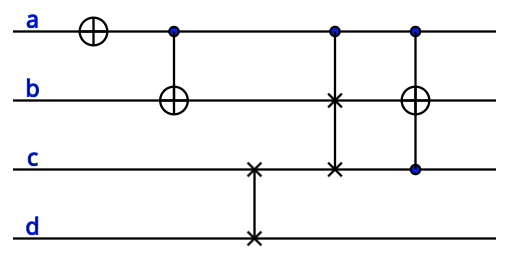
\includegraphics[width=500px]{figures/fig_reversible_gates.png}}

\end{edXtext}

%%%%%%%%%%%%%%%%%%%%%%%%%%%%%%%%%%%%%%%%

\begin{edXproblem}{Reversible two-four-three swap}{url_name=u1_1_four_input_cswap attempts=20}

\edXincludepy{lib/ftdigital2.py}

Design a reversible circuit, using NOT, CNOT, Toffoli, and Fredkin gates, which acts on the four inputs $a, b, c, d$, to perform the operation
${\rm swap_{243}}(a,b,c,d)$ which swaps $b$ and $d$ if $a=0$, and swaps $c$ and $d$ if $a=1$.  Bit $a$ should be left unchanged.

Note that you have 20 attempts, so you have some leeway with syntax
mistakes.  Most later problems will just provide 10.  Work out your
circuits in your own notebook and check carefully before entering; do
not rely on random exploration to get the correct answer.

\edXabox{type="custom" 
  rows=8   
  expect=""
  cfn="check_243_swap" 
  % math=1 
  % inline="1"
}


\begin{edXsolution}

  One correct solution is:
\begin{verbatim}
fredkin(a,c,d)
not(a)
fredkin(a,b,d)
not(a)
\end{verbatim}

\centerline{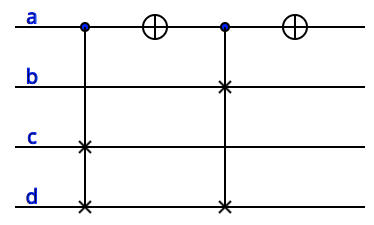
\includegraphics[width=500px]{figures/ps1a_swap243_circuit.png}}

\end{edXsolution}

\edXaskta{}

\end{edXproblem}

\AddSearchBox{001100}


\end{edXvertical}

%%%%%%%%%%%%%%%%%%%%%%%%%%%%%%%%%%%%%%%%

\begin{edXvertical}{Controlled-controlled swap}

\begin{edXproblem}{Controlled-controlled swap}{url_name=u1_1_ccswap attempts=10}

\edXincludepy{lib/ftdigital2.py}

Design a reversible circuit, using NOT, CNOT, Toffoli, and Fredkin gates, which acts on the four inputs $a, b, c, d$, to swap $c$ and $d$ only when both $a=1$ and $b=1$.  You may use a fifth bit $e$, given as initialized to $e=0$, in your circuit; this bit must also end as $e=0$.

\edXabox{type="custom" 
  % size=70   
  rows=8   
  expect=""
  cfn="check_ccswap" 
  % math=1 
  % inline="1"
}


\begin{edXsolution}

  One correct solution is:

\begin{verbatim}
fredkin(a,b,e)
fredkin(e,c,d)
fredkin(a,b,e)
\end{verbatim}

\centerline{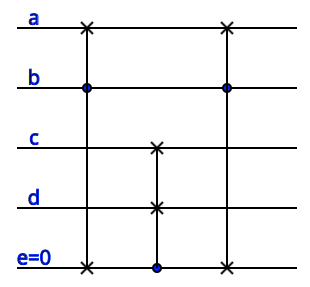
\includegraphics[width=500px]{figures/ps1a_ccswap_circuit.png}}

\end{edXsolution}

\edXaskta{}

\end{edXproblem}

\AddSearchBox{001101}

\end{edXvertical}

%%%%%%%%%%%%%%%%%%%%%%%%%%%%%%%%%%%%%%%%

\begin{edXvertical}{Reversible two-input demultiplexer}

\begin{edXproblem}{Reversible two-input demultiplexer}{url_name=u1_1_demux2 attempts=10}

\edXincludepy{lib/ftdigital2.py}

Design a reversible circuit, using NOT, CNOT, Toffoli, and Fredkin
gates, which acts on the two arbitrary inputs $a, b$, and the two
fixed inputs $c=0$, $d=0$, to produce four bits $a'$, $b'$, $c'$, $d'$
of output, where only the $n^{\rm th}$ output is $1$
(the others are all $0$), and $n=2b + a$.

This is a two-input demultiplexer, and the output is a unary encoded
value, sometimes otherwise known as \href{https://en.wikipedia.org/wiki/One-hot}{``one-hot encoding''} in the field
of deep neural networks.

\begin{edXshowhide}{Hint}
Denoting the NOT of $a$ as $\bar{a}$, note that
\bea
  a' &=& \bar{a} \bar{b} \\
  b' &=& a\bar{b} \\
  c' &=& \bar{a}b \\
  d' &=& ab
\,.
\eea

Since these are all Boolean functions of the input, it would seem
immediate how to compute these using Boolean logic functions.  The
trick here is that you're being asked to construct the circuit using
reversible gates, consuming no additional inputs, and producing no
extra garbage.  This is known as an ``in-place'' reversible circuit.

You should be able to do this using 11 gates.  If you can do it with fewer, let the TA know!
\end{edXshowhide}

\edXabox{type="custom" 
  % size=70   
  rows=8   
  expect=""
  cfn="check_demux2" 
  % math=1 
  % inline="1"
}

\begin{edXsolution}
  A reasonable solution is:

\begin{verbatim}
		toffoli(a,b,d)
		not(a)
                toffoli(a,b,c)
                not(a)
                cnot(d,b)
                cnot(c,b)
                not(d)
                toffoli(a,d,b)
                not(d)
                not(a)
                cnot(c,a)
\end{verbatim}

\centerline{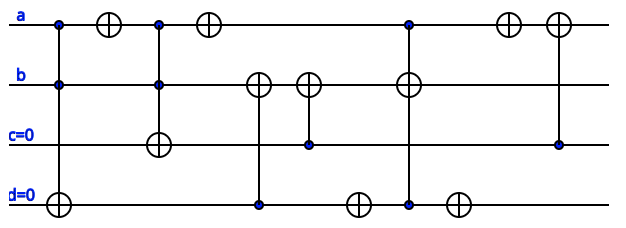
\includegraphics[width=500px]{figures/ps1a_demux2_circuit.png}}
  
\end{edXsolution}

\edXaskta{}

\end{edXproblem}

\AddSearchBox{001101}

\end{edXvertical}

%%%%%%%%%%%%%%%%%%%%%%%%%%%%%%%%%%%%%%%%
\end{edXsection}


